\documentclass{article}


\usepackage{longtable}
\usepackage[margin=1in]{geometry}
\usepackage[section]{placeins}
\usepackage{cite}

\title{Improving Day Ahead Electricity Load Forecasts with Google Trends}
\author{Cameron Mulder\\ James Woods}

% \date{}
 

\usepackage{Sweave}
\begin{document}
\maketitle
\setkeys{Gin}{width=0.7\textwidth}


\begin{abstract}
Modern short term load forecasting has grown in analytically complexity and sophistication.  Day ahead forecasts now commonly use neural nets, Monte Carlo simulations and a wealth of historical data.  What they have not done is fully captured the sentiment and intentions of the people using the electricity.  This paper introduces Google Trend data, a summary of Google searches, as a way of capturing this sentiment and refining forecasts.  We show with drop all forward cross validation that this amendment decreases forecast uncertainty by approximately 5\% when compared to a statistically adjusted forecast and by over 50\% when compared to raw forecasts.
\end{abstract}

\Sconcordance{concordance:DraftPaper.tex:DraftPaper.Rnw:%
1 14 1 1 0 13 1 1 9 13 1 1 11 7 1 1 8 1 2 7 1 1 8 1 2 18 1 1 11 1 3 9 1 %
1 11 1 3 19 1 1 23 2 1 1 9 5 1 1 9 1 2 5 1 1 15 7 1 1 25 1 1 1 5 35 0 1 %
2 18 1 1 13 42 0 1 2 9 1 1 3 32 0 1 1 32 0 1 1 32 0 1 1 32 0 1 1 32 0 1 %
1 32 0 1 2 1 1 1 2 32 0 1 1 32 0 1 1 32 0 1 1 32 0 1 1 32 0 1 1 32 0 1 %
3 1 1 1 3 32 0 1 1 32 0 1 1 32 0 1 1 32 0 1 1 32 0 1 1 32 0 1 2 2 1 1 3 %
32 0 1 1 32 0 1 1 32 0 1 1 32 0 1 1 32 0 1 1 32 0 1 7 5 1}


\section{Introduction}



\begin{enumerate}
  \item Intro to short term load forecasting.
  \item Why crowd sourced, non technical,  information could be useful.
  \item Google trends is the summation of Google searches.
  \item Outline of paper
\end{enumerate}


\section{Data Sources}

  \subsection{PJM Load Forecasts and Actuals}
  
  





\begin{figure}
\begin{center}
\caption{Confidence Intervals for Intercept Statistically Adjusted Models (95\%)}
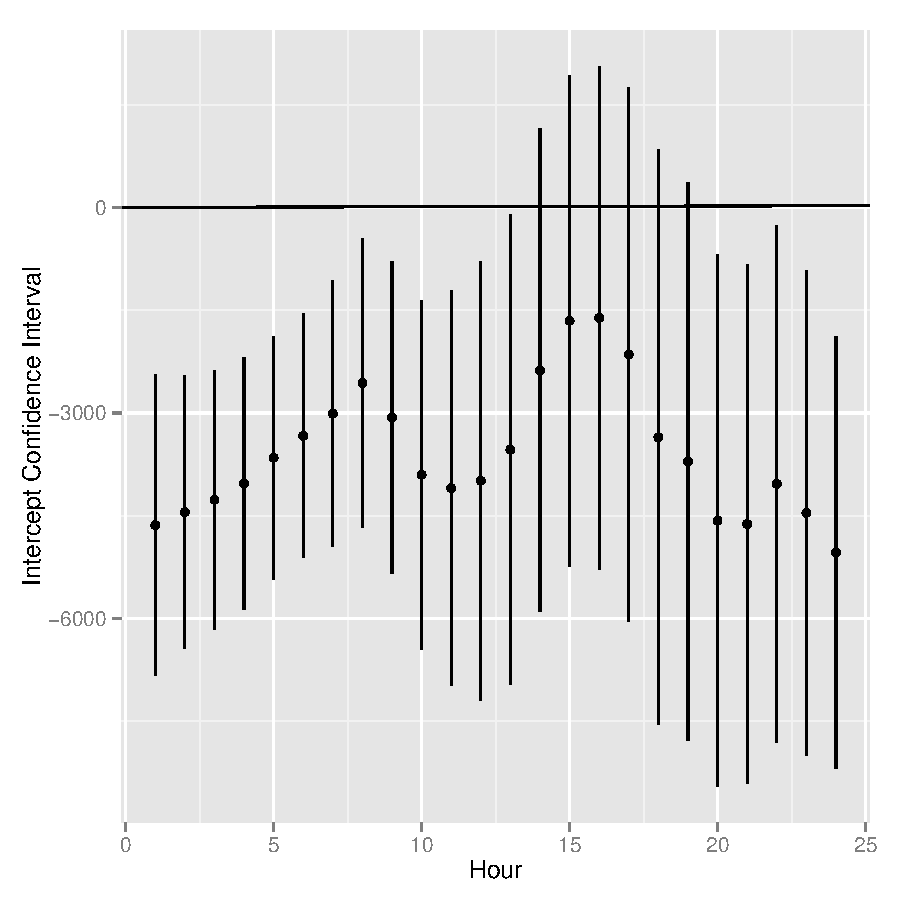
\includegraphics{DraftPaper-003}
\end{center}
\end{figure}



\begin{figure}
\begin{center}
\caption{Confidence Intervals for Co-Movement Statistically Adjusted Models (95\%)}
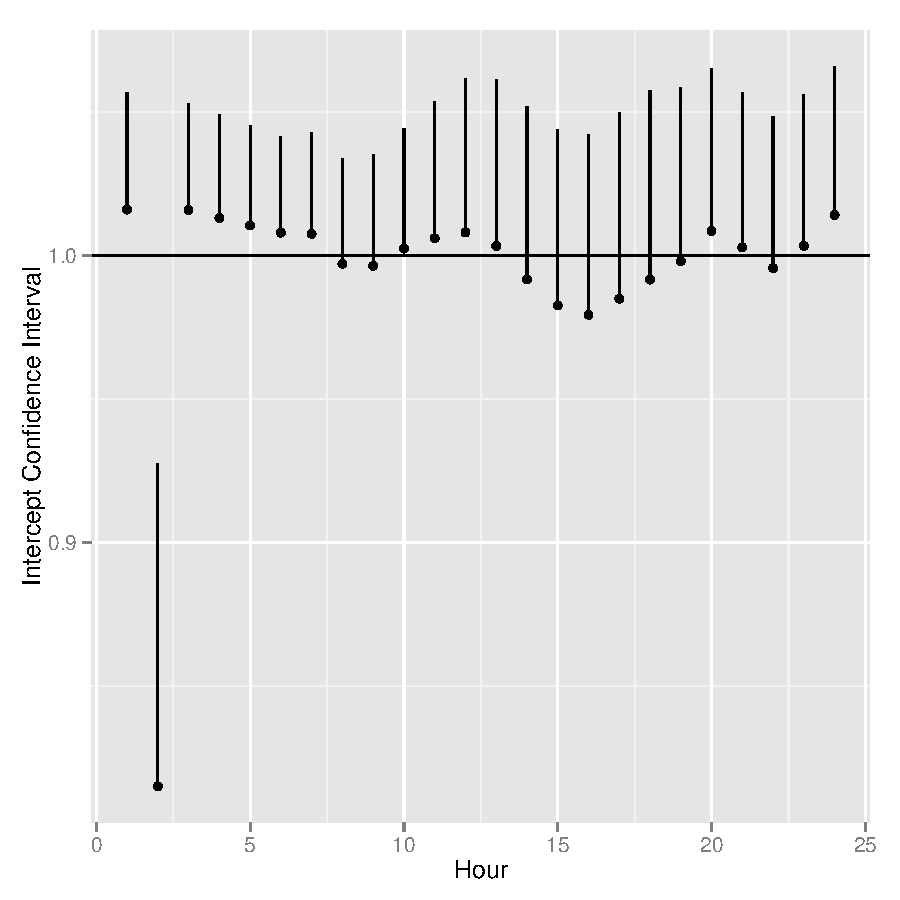
\includegraphics{DraftPaper-004}
\end{center}
\end{figure}




    \begin{enumerate}
      \item Data sources.
      \item Documentation of forecasting.
      \item Forecast bias
      \item Statistically adjusted forecasts.
      \item Note that almost all hours are biased and that co-movements are good for peak hours
    \end{enumerate}

  \subsection{Google Trends}

\begin{figure}
\begin{center}
\caption{State Weather Trends Indexes Over Time}
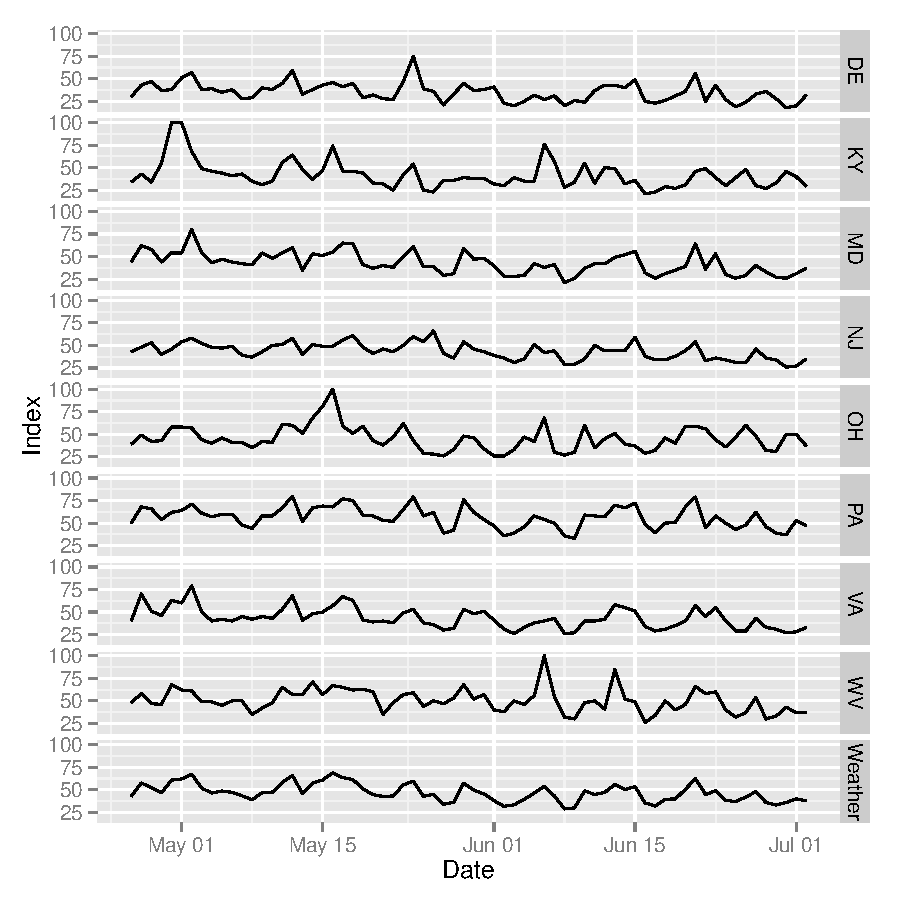
\includegraphics{DraftPaper-005}
\end{center}
\end{figure}





\begin{figure}
\begin{center}
\caption{Trends Indexes Over Time}
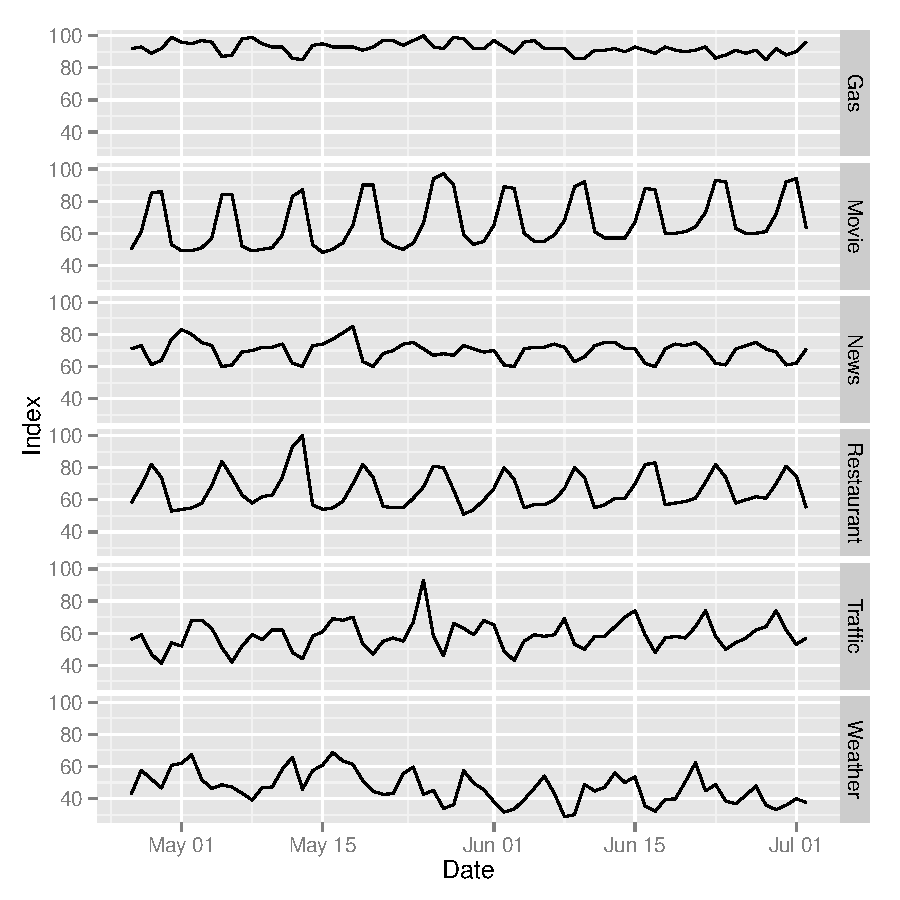
\includegraphics{DraftPaper-006}
\end{center}
\end{figure}



    \begin{enumerate}
      \item Where to get the data
      \item Limitations
      \item Forming a population weighted index.
      \item Other common searches that will be used as counter examples.
    \end{enumerate}

\section{Post Forecast Addition of Google Trends Data}

  \begin{enumerate}
    \item Simple hourly models with Trends.
    \item Gross comparison with actual forecast and statistically adjusted forecasts.
    \item Why this is insufficient.
  \end{enumerate}







\begin{figure}
\begin{center}
\caption{Confidence Intervals for ``Weather'' in Trends Models (95\%)}
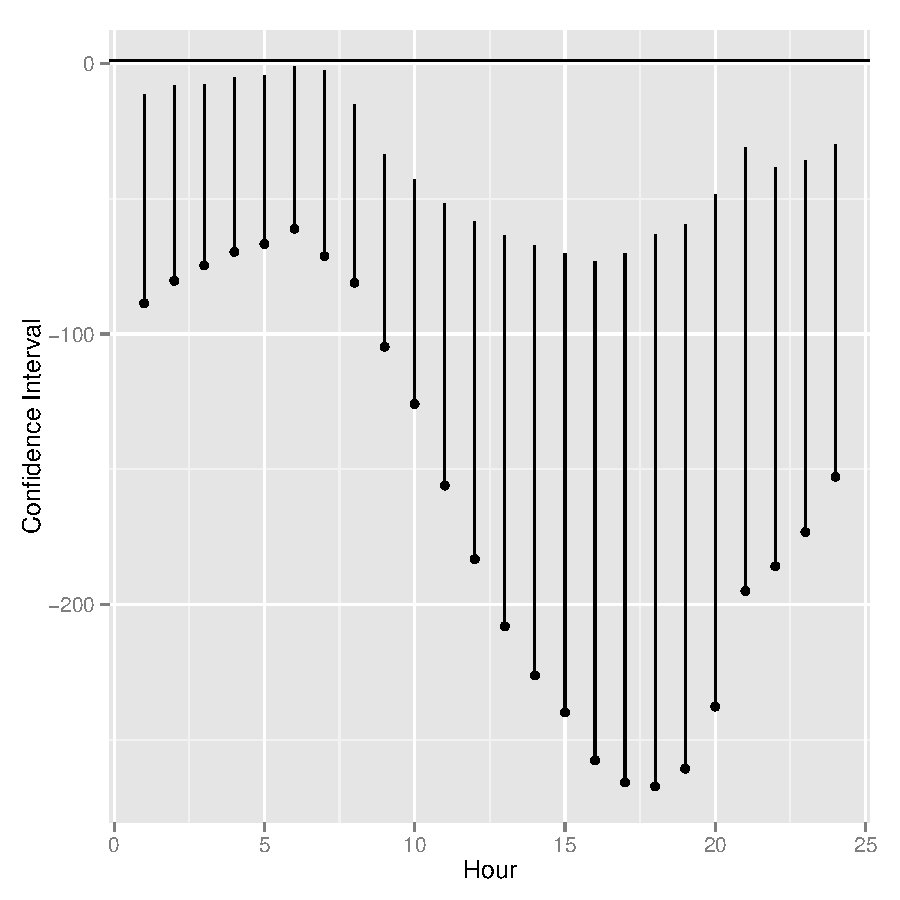
\includegraphics{DraftPaper-009}
\end{center}
\end{figure}



  






  \subsection{Drop Forward Cross-validation}


  
% Table created by stargazer v.5.1 by Marek Hlavac, Harvard University. E-mail: hlavac at fas.harvard.edu
% Date and time: Wed, Jul 30, 2014 - 11:11:12 AM
\begin{table}[!htbp] \centering 
  \caption{Improvement in Forecasts Relative to Gross,  Statistically Adjusted, Drop Forward CV (Percent)} 
  \label{} 
\begin{tabular}{@{\extracolsep{5pt}} cccc} 
\\[-1.8ex]\hline 
\hline \\[-1.8ex] 
Hour & Direct & Statistically Adjusted (Raw) & Statistically Adjusted (CV) \\ 
\hline \\[-1.8ex] 
$1$ & $3.914$ & $4.091$ & $4.561$ \\ 
$2$ & $30.473$ & $3.615$ & $4.467$ \\ 
$3$ & $50.565$ & $3.628$ & $4.779$ \\ 
$4$ & $60.402$ & $3.138$ & $4.444$ \\ 
$5$ & $66.381$ & $3.049$ & $4.089$ \\ 
$6$ & $73.314$ & $2.382$ & $4.075$ \\ 
$7$ & $79.050$ & $2.627$ & $4.632$ \\ 
$8$ & $82.113$ & $5.250$ & $6.716$ \\ 
$9$ & $78.317$ & $9.197$ & $10.984$ \\ 
$10$ & $72.175$ & $9.969$ & $10.989$ \\ 
$11$ & $67.881$ & $9.630$ & $9.518$ \\ 
$12$ & $67.577$ & $9.133$ & $7.772$ \\ 
$13$ & $68.331$ & $8.662$ & $6.620$ \\ 
$14$ & $70.287$ & $8.362$ & $6.088$ \\ 
$15$ & $71.514$ & $8.199$ & $5.456$ \\ 
$16$ & $71.155$ & $7.934$ & $5.313$ \\ 
$17$ & $70.310$ & $7.292$ & $5.068$ \\ 
$18$ & $68.395$ & $6.504$ & $4.612$ \\ 
$19$ & $66.234$ & $6.252$ & $4.594$ \\ 
$20$ & $63.033$ & $5.638$ & $2.361$ \\ 
$21$ & $61.587$ & $4.634$ & $1.415$ \\ 
$22$ & $61.377$ & $5.712$ & $3.784$ \\ 
$23$ & $55.833$ & $5.727$ & $3.730$ \\ 
$24$ & $50.531$ & $5.480$ & $3.274$ \\ 
\hline \\[-1.8ex] 
\end{tabular} 
\end{table}   
  
  
    \begin{enumerate}
      \item Cross validation concepts.
      \item Why drop forward cross validation is the right concept.
      \item Comparison of drop forward statistically adjusted and Trends adjusted with gross comparisons.
      \item Reiteration that comparison with raw forecasts is a slam dunk.
    \end{enumerate}
    
  \subsection{Counter-factual Test with Other Common Google Searches}
  
  
  
    \begin{enumerate}
      \item Comparison with: news, recipe, traffic, gas.
      \item Note that some of them kinda work.
    \end{enumerate}
    
% Table created by stargazer v.5.1 by Marek Hlavac, Harvard University. E-mail: hlavac at fas.harvard.edu
% Date and time: Wed, Jul 30, 2014 - 11:11:13 AM
\begin{table}[!htbp] \centering 
  \caption{Alternate Google Search Models for Hour 19} 
  \label{} 
\begin{tabular}{@{\extracolsep{5pt}}lccccc} 
\\[-1.8ex]\hline 
\hline \\[-1.8ex] 
 & \multicolumn{5}{c}{Hour 19 Load} \\ 
\cline{2-6} 
 & News & Gas & Traffic & Restaurant & Movie \\ 
\\[-1.8ex] & (1) & (2) & (3) & (4) & (5)\\ 
\hline \\[-1.8ex] 
 F19 & 0.942$^{***}$ & 0.971$^{***}$ & 0.952$^{***}$ & 0.956$^{***}$ & 0.940$^{***}$ \\ 
  & (0.039) & (0.038) & (0.041) & (0.037) & (0.038) \\ 
  & & & & & \\ 
 NewsTrends & $-$165.209$^{**}$ &  &  &  &  \\ 
  & (69.522) &  &  &  &  \\ 
  & & & & & \\ 
 GasTrends &  & $-$97.010 &  &  &  \\ 
  &  & (106.696) &  &  &  \\ 
  & & & & & \\ 
 TrafficTrends &  &  & $-$69.267 &  &  \\ 
  &  &  & (44.882) &  &  \\ 
  & & & & & \\ 
 RestaurantTrends &  &  &  & 90.097$^{**}$ &  \\ 
  &  &  &  & (35.645) &  \\ 
  & & & & & \\ 
 MovieTrends &  &  &  &  & 71.976$^{***}$ \\ 
  &  &  &  &  & (26.775) \\ 
  & & & & & \\ 
 Constant & 17,443.060$^{**}$ & 11,951.160 & 8,913.360 & $-$1,400.642 & 1,282.578 \\ 
  & (7,432.784) & (11,632.000) & (5,896.900) & (3,912.481) & (3,557.924) \\ 
  & & & & & \\ 
\hline \\[-1.8ex] 
Observations & 68 & 68 & 68 & 68 & 68 \\ 
Log Likelihood & $-$624.411 & $-$626.318 & $-$626.431 & $-$624.767 & $-$624.639 \\ 
Akaike Inf. Crit. & 1,258.821 & 1,262.637 & 1,262.863 & 1,259.535 & 1,259.278 \\ 
Bayesian Inf. Crit. & 1,269.693 & 1,273.509 & 1,273.735 & 1,270.406 & 1,270.150 \\ 
\hline 
\hline \\[-1.8ex] 
\textit{Note:}  & \multicolumn{5}{r}{$^{*}$p$<$0.1; $^{**}$p$<$0.05; $^{***}$p$<$0.01} \\ 
\end{tabular} 
\end{table} 


\section{Summary and Conclusions}


\appendix

\section{Hourly Models with Weather Searches}

\clearpage



% \bibliography{Trends.bib}
% \bibliographystyle{apalike}

\end{document}
